% !TeX root = ../praktikum.tex
% !TeX encoding = UTF-8
% !Tex spellcheck = de_DE

\subsection{Lichtsensor}
Um aus dem Spannungsabfall über den zu der Photodiode parallel geschalteten Widerstand eine Lichtleistung bestimmen zu können ist ein lineares Verhalten von Vorteil. So kann direkt aus der Spannung mittels eines Faktors die Leistung berechnet werden. Mit einem Widerstand von $\unit[1]{k\Omega}$ ist ein lineares Verhalten nur im Bereich bis etwa \unit[0,7]{mW} zu beobachten. Darüber hinaus sättigt die Spannung. Vermutlich ließe sich mit einer Wertetabelle (erstellt mit Hilfe des kommerziellen Powermeters) auch weit über diesen Bereich hinaus sinnvoll die Lichtleistung berechnen.

Für den $\unit[500]{\Omega}$ Widerstand ist bis zur maximal vermessenen Lichtleistung $P_L$ von etwa \unit[1,1]{mW} keine Sättigung festzustellen (vgl. Abb.~\ref{fig:photodiode}). Für den vorgesehen Verwendungszweck empfiehlt sich daher die Verwendung eines Widerstandswertes in der Nähe von $\unit[500]{\Omega}$. Mit Hilfe der Software \textit{QtiPlot} wurde eine Lineare Regression mit der Formel $U=a\cdot P_L + b$ über die aufgenommenen Datenpunkte ausgeführt. Daraus ergeben sich die Werte $b=(5,2346 \pm 1,1515) \unit{mW} $ und $a= 152,6614\pm 1,7095) \unitfrac{W}{V}$. Die Standardabweichung liegt bei $1,28$.\\


Das beobachtet Verhalten lässt sich sehr gut erklären, indem man einen PN-Übergang in der Photodiode mit einer Bandlücke von etwa \unit[500]{mV} annimmt. Für eine feste Frequenz kann die Lichtleistung direkt in die Anzahl der Photonen $N_{Ph}$ umgerechnet werden: $N_{Ph} = \nicefrac{P_L}{E_{Ph}}$, wobei $E_{Ph}=\hbar \omega_{Ph}$ die Energie pro Photon ist. Jedes dieser Photonen treibt mit einer Wahrscheinlichkeit, entsprechend der Quanteneffizienz des Überganges für die Frequenz der Photonen $\omega_{Ph}$, genau einen elektronischen Übergang. So führt eine bestimmt Leistung zu einer bestimmten Anzahl angeregter Elektronen. Dies entspricht bei kompletter Besetzungsinversion der Zustände einem konstantem Strom und somit Spannungsabfall über den Widerstand. Sobald dieser Widerstand jedoch so groß gewählt wird, dass der Spannungsabfall in etwa dem Bandlückenpotential entspricht, wird die Besetzungsinversion aufgehoben. Dadurch sinkt die Quanteneffizienz und folglich der Stromfluss. Folglich sinkt die abgefallene Spannung über den Widerstand. Dies erklärt das lineare Verhalten bei kleinen Widerständen beziehungsweise Lichtleistungen und das Sättigungsverhalten ab etwa \unit[250]{mV}.

\subsection{Erzeugung von Beugungsbilder von verschiedenen Gittern}

In diesem Versuchsteil wurden in der Abbildungsebene vertikale und Kreuzgitter im 4f-Aufbau mit einer größtmöglichen Schärfe erzeugt (Abb.~\ref{fig:gitter_und_spektrum}~a), \ref{fig:kreuzgitter_und_spektrum}~a). %Gitter sind Objekte, die aus Einzelspalten in gleichmäßigen Abständen zusammengesetzt sind.
Da das Licht im vertikalen Gitter nur in der vertikalen Richtung gebeugt wird, bilden sich die Intensitätsschwankungen in der Fourierebene ausschließlich in horizontaler Richtung aus. Somit wurde dort eine senkrecht zu dem Gitter stehende Punktreihe aus Interferenzmaxi- und -minima (Abb.~\ref{fig:gitter_und_spektrum}) beobachtet werden, vergleich Abbildung~\ref{fig:gitter_und_spektrum}.
	
\begin{figure}[ht]
	\centering
	%\includegraphicsRS[width=0.6\textwidth]{images/Regina/abb13.jpg}
	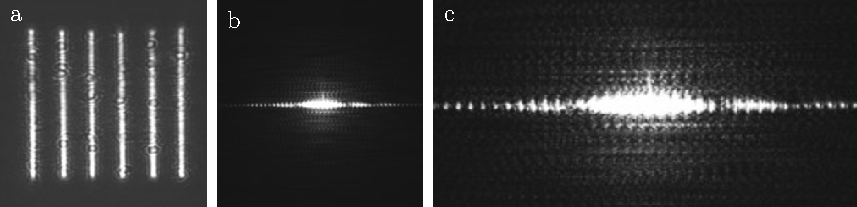
\includegraphics{images/Regina/abb13.pdf}
	\caption[Gitter mit Fourierspektrum]{
		Vertikales Gitter (a) und das dazugehörige Beugungsbild (b), welches das Fourierspektrum darstellt. Das Fourierspektrum weist erneut Beugungsbilder als eine Unterstruktur auf (c).
	}
	\label{fig:gitter_und_spektrum}
\end{figure}


Bei einem Kreuzgitter findet die Beugung folglich in horizontaler und vertikaler Richtung statt, welches einer Kreuzform in der Fourierebene entspricht. Unser erster Versuch ergab in der Fourierebene die in Abbildung~\ref{fig:kreuzgitter_und_spektrum}~c) dargestellt kreuzförmige Anordnung, die jedoch nicht ein einzelnes Kreuz, sondern mehrere Kreuze mit einem bestimmten Abstand voneinander darstellte. Da das Verschiebungstheorem der Fouriertransformation besagt (siehe 1.1. Verschiebung%TODO:REF!!!
), dass die unterschiedliche Position der einzelnen Spalte keinen Einfluss auf das Beugungsbild hat, solange sich das Objekt im Lichtstrahl befindet und somit vollständig ausgeleuchtet ist, konnte dieses Fourierspektrum nicht nur durch ein einziges Kreuzgitter erzeugt worden sein. 

\begin{figure}[ht]
	\centering
	%\includegraphicsRS[width=0.4\textwidth]{images/Regina/abb14.jpg}
	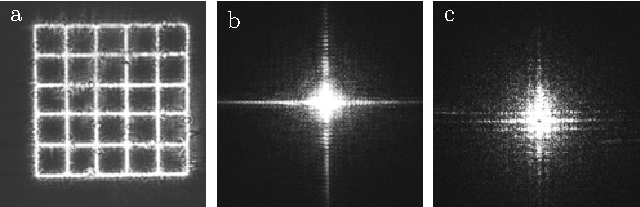
\includegraphics{images/Regina/abb14.pdf}
	\caption[Kreuzgitter mit Fourierspektrum]{
		Kreuzgitter (a) und das dazugehörige Beugungsbild (b), das das Fourierspektrum darstellt. Eine Überlagerung von mehreren Fourierspektren (c).
	}
	\label{fig:kreuzgitter_und_spektrum}
\end{figure}

Da wir in der Objektebene ein Dia als Quelle unserer Abbildungen verwendet haben und dieses Dia wie in Abb. 8%TODO REF!!!
 dargestellt (Objekt 3) in der untersten Reihe drei verschiedene Kreuzgitter und darüber weitere horizontale und vertikale Gitter aufwies, wurden diese ebenfalls angestrahlt und lieferten die zusätzlichen Kreuze. Um diese zu unterbinden, wurden die anderen Objekte, auch bei den nachfolgenden verwendeten Objekten, mit schwarzen Klebeband überklebt. Durch diese Modifizierung der Dias konnte das erwartete einzige Kreuz erzeugt werden (Abb.~\ref{fig:gitter_und_spektrum}~b).

Sowohl bei dem vertikalen Gitter als auch bei dem Kreuzgitter ist in der Fourierebene im Zentrum der Beugungsbilder eine maximale Intensität zu erkennen. Dieses Maximum entsteht durch das Kreuzen der mittleren horizontalen oder im Kreuzgitter der vertikalen und
horizontalen Beugungsbilder. Dabei ist bei jedem weiteren Kreuzpunkt erneut eine erhöhte Intensität zu erkennen, die aber nach außen hin abnimmt. Diese lässt sich ebenfalls bei einem
Doppelspalt beobachten, wobei das Intensitätsmaximum nullter Ordnung am stärksten ist und die Maxima höherer Ordnungen immer schwächer werden ($\nicefrac{sin(x)}{x}$). Dabei nimmt die Intensität im Zentrum mit zunehmen kleiner werdenden Gitterkonstante zu.
Weiterhin wiesen alle Intensitätsmaxima eine Unterstruktur auf. Diese Unterstrukturen entstehen durch die Interferenz der Haupt- und Nebenmaxima aller Spalte des Gitters. Somit entsteht im Gegensatz zu einem Doppelspalt das Beugungsbild eines Gitter aus Vielfachinterferenzen. Diese Eigenschaft entspricht der mathematischen geforderten Linearität. Denn das Beugungsbild eines Gitters kann somit durch das aufsummieren der einzelnen Beugungsbilder des Einzelspaltes erzeugt werden (siehe 1.1. Linearität%TODO:REF!!!
).

\subsection{Erzeugung von Beugungsbilder von Punkten}

Bei der optische Fouriertransformation gilt für Punkte wie bereits für Gittern erläutert die Linearität, so dass das erzeugte Beugungsbild in der Fourierebene sich aus der Summe der Beugungsbilder der einzelnen Punkte ergibt. Das Beugungsbild eines Punktes besteht aus konzentrischen Ringen, dessen Breite und Intensität nach außen abnehmen. Durch das Verschiebungtheorem der Fouriertransformation ist gegeben, dass sich das Beugungsbild der beiden Punkte an einer Position befinden, trotz der unterschiedlichen Position der Punkte. Bei zwei Punkten ergibt sich somit erneut eine Vielfachinterferenz analog zum Gitter, welches erneut durch Unterstrukturen in den konzentrischen Ringen erkennbar wird (Abb.~\ref{fig:punktpaare_verschieden_und_spektren}~b, d). Mit zunehmenden Abstand zwischen den Punkten werden die Unterstrukturen feiner. Dieses entspricht dem Ähnlichkeitstheorem (siehe 1.1. Ähnlichkeit%TODO:REF!!!
), so dass mit zunehmenden Abständen der Punkte sich die Beugungsmaxima annähern, bzw. die Abstände zwischen diesen kleiner werden. Für ein Gitter bedeutet dieses, je größer die Gitterkonstante ist, d.h. je größer der Abstand zwischen den Spalten ist, desto kleiner wird der Abstand zwischen den einzelnen Maxima und Minima.

\begin{figure}[h]
	\centering
	%\includegraphicsRS[width=0.3\textwidth]{images/Regina/abb15.jpg}
	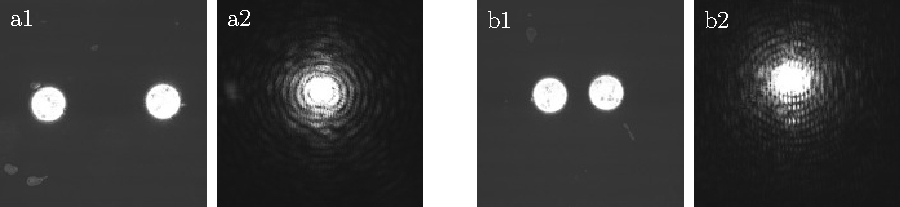
\includegraphics{images/Regina/abb15.pdf}
	\caption[Punktpaare unterschiedlicher Abstände und Fourierspektren]{
		Punktpaare mit unterschiedlichen Abständen zueinander (a1, b1) und die dazugehörigen Beugungsbilder in der Fourierebene (a2, b2).
	}
	\label{fig:punktpaare_verschieden_und_spektren}
\end{figure}


\begin{figure}[h]
	\centering
	%\includegraphicsRS[width=0.3\linewidth]{images/Regina/abb16.jpg}
	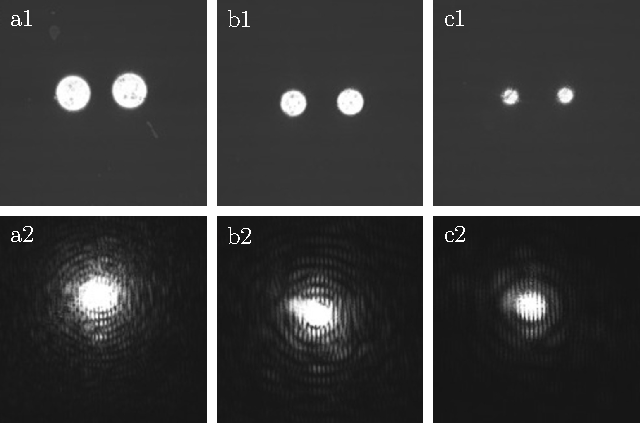
\includegraphics{images/Regina/abb16.pdf}
	\caption[Punktpaare gleicher Abstände und Fourierspektren]{
		Punktpaare mit gleichen Abständen und unterschiedlicher Größe (a1, b1, c1) und die dazugehörigen Beugungsbilder in der Fourierebene (a2, b2, c2).
	}
	\label{fig:punktpaare_gleich_und_spektren}
\end{figure}

Bei den geringsten Abstand sind im Beugungsbild neben den konzentrischen Formen auch vertikale Gitter zu erkennen (Abb.~\ref{fig:punktpaare_verschieden_und_spektren}~b2). Diese Gitterform stellen die bereits erwähnten Unterstrukturen der Beugungsbilder dar. Zwei Punkte ergeben in der Fourierebene als
Unterstruktur eine Linienstruktur senkrecht zur Verbindungslinie der beiden Punkte. Diese ergeben sich somit ebenfalls bei zwei Punkten mit höheren Abstand, sind aber wegen des kleinen Abstand zwischen den Spalten des vertikalen Gitters in der Fourierebene schlecht zu erkennen, da sich die Fouriertransformierte reziprok verhält (Ähnlichkeitstheorem). Bei kleinere Abstand zwischen den Punkten, vergrößert sich der Abstand der Spalten im vertikalen Gitter, und ist dadurch erkennbar. Diese Unterstrukturen sind noch ausgeprägter bei gleichbleibenden Abstand und kleinerer Größe der Punkte zu erkennen (Abb.~\ref{fig:punktpaare_gleich_und_spektren}~b2, c2). Die Intensitätsmaxima sind bei den kleineren Punkte durch ihren größeren Abstand zueinander kleiner ausgeprägt als bei den größeren Punkten. Somit weist das Hauptmotiv des Beugungsbild eine geringe Intensität auf, wodurch die Unterstruktur einfacher zu erkennen
ist.
Auch bei dem Beugungsbild eines Punktringes (Abb.~\ref{fig:punktringe_und_spektrum}) sind Unterstrukturen in der Fourierebene zu erkennen, die sich durch die Anordnung der acht Punkte ergeben. Zwei Punkte weisen eine senkrechte Linienstruktur zur Verbindungslinie auf, so dass sich bei acht Punkten vier Linienstrukturen (horizontal, vertikal, beide Diagonale) ergeben. Wenn sich diese Strukturen kreuzen, ergeben sich acht Schnittpunkte und somit eine Unterstrukturen, die wie Achtecke aussehen (Abb.~\ref{fig:punktringe_ausschnitt}).

\begin{figure}[h]
	\centering
	%\includegraphicsRS[width=0.10\linewidth]{images/Regina/abb17.jpg}
	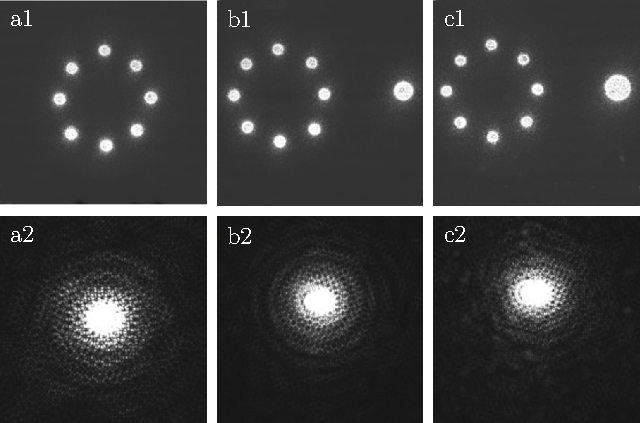
\includegraphics{images/Regina/abb17.pdf}
	\caption[Punktringe mit Fourierspektren]{
		Punktringe (a1) und Punktringe mit zusätzlichem Punkt in unterschiedlicher Größe (b1, c1) und die dazugehörigen Beugungsbilder in der Fourierebene (a2-c2).
	}
	\label{fig:punktringe_und_spektrum}
\end{figure}

\begin{figure}[h]
	\centering
	\includegraphicsRS[width=0.50\textwidth]{images/Regina/abb18.jpg}
	\caption[Beugungsbild der Punktringe mit vergrößertem Ausschnitt]{
		Ausschnitt aus dem Beugungsbild des Punktringes, welche die Unterstruktur eines Achtecks zeigt.
	}
	\label{fig:punktringe_ausschnitt}
\end{figure}

Bei einem Punktkreis mit einem zusätzlichen Punkt ist das Beugungsbild nicht mehr symmetrisch und die Asymmetrie nimmt mit größer werdenden Punkt zu (Abb.~\ref{fig:punktpaare_gleich_und_spektren}~b, c).


\subsection{Erzeugung von Beugungsbilder von Buchstaben und Zahlen}

Der Buchstabe D besteht aus sowohl horizontalen, vertikalen Linien und runden Elementen (Abb.~\ref{fig:ziffern_mit_spektren}~a1). Das Beugungsbild ergibt sich somit aus der Summe der Beugungsbilder dieser verschiedenen Formen. Die horizontalen Linien bilden ein Fourierspektrum in der Horizontalen und die vertikalen Linien in der Vertikalen mit den jeweiligen Maxima und Minima und Unterstrukturen (Abb.~\ref{fig:ziffern_mit_spektren}~a2). Die runde Form erzeugt in dem Beugungsbild konzentrische Ringe mit abnehmender Intensität, entsprechend dem Beugungsbild von Punkten. Da der Buchstabe D durch horizontale und vertikalen Linien dominiert wird, ist auch das Beugungsbild stark davon geprägt, so dass die konzentrischen Ringe durch eine geringere Intensität auch schlechter zu erkennen sind.

\begin{figure}[h]
	\centering
	%\includegraphicsRS[width=0.4\textwidth]{images/Regina/abb19.jpg}
	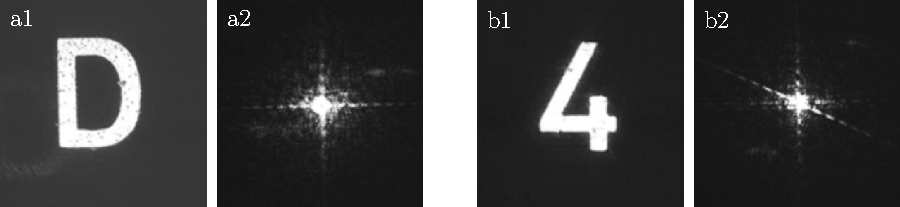
\includegraphics{images/Regina/abb19.pdf}
	\caption[Ziffern mit Fourierspektren]{
		Buchstabe D (a1) und Zahl 4 (b1) und die dazugehörigen Beugungsbilder in der Fourierebene (a2 und b2).
	}
	\label{fig:ziffern_mit_spektren}
\end{figure}

Die Zahl 4 besteht lediglich aus Linien, wobei neben horizontalen und vertikalen Linien ebenfalls diagonale Linien vorhanden sind (Abb.~\ref{fig:ziffern_mit_spektren}~b1). Da das erzeugten Beugungsbild eines Gitters eine senkrecht auf dem Gitter stehende Punktereiche aus Interferenzmaxima und –minima darstellt, ist zusätzlich zu der horizontalen und vertikalen Richtung ein Fourierspektrum in der Diagonalen senkrecht zur der Diagonale der Objektebene anzufinden (Abb.~\ref{fig:ziffern_mit_spektren}~b2).

\subsection{Erzeugung von Beugungsbildern des Fourierhauses}

Das Fourierhaus ist ein Haus, welches aus Gittern mit gleichen Gitterkonstanten und unterschiedlicher Ausrichtungen der Gitter besteht (Abb.~\ref{fig:fourierhaus_mit_filtern}~a1). Die verschiedenen Gitter entsprechen verschiedenen Bauelementen im Haus. Die Wand besteht aus einem vertikalen Gitter, das Dach aus einem horizontalen Gitter und die Tür und der Schornstein werden aus diagonalen Gittern in entgegen gerichteten Richtung erstellt. Die Fouriertransformation dieses Fourierhauses ergibt das in Abbildung~\ref{fig:fourierhaus_mit_filtern}a2 dargestellte Beugungsbild. Die vier verschiedenen Orientierung der Gitter sind in der Fourierebene ebenfalls durch vier verschiedene Orientierungen dargestellt, die jeweils senkrecht auf der Objektebene stehen. Da die Gitterkonstante des Fourierhauses im Vergleich zu den in Abbildung~\ref{fig:gitter_und_spektrum} und \ref{fig:kreuzgitter_und_spektrum} gezeigten Gittern sehr viel kleiner ist, sind die Abstände zwischen den Maxima im Fourierspektrum deutlich größer (siehe 1.1. Ähnlichkeit%TODO REF!!!
 ) und die Intensität im Zentrum erhöht.

\begin{comment}
%Bild wurde mit in das nächste eingebaut.
\begin{figure}[h]
	\centering
	\includegraphicsRS[width=0.4\textwidth]{images/Regina/abb20.jpg}
	\caption[Fourierhaus mit Fourierspektrum]{
		Das Fourierhaus   bestehend aus Gittern verschiedener Ausrichtungen, die 	verschiedene Bauteile des Hauses darstellen (a) und die dazugehörigen Beugungsbilder in der Fourierebene (b).
	}
	\label{fig:fourierhaus_und_spektrum}
\end{figure}
\end{comment}

\subsection{Optische Filterung des Fourierhauses durch eine Schneide}

Für eine optische Filterung wurden verschiedene Filter in der Fourierebene des 4f-Aufbaus eingesetzt (siehe Abb.4%TODO:REF!!!
). Zuerst wurde das Fourierhaus durch Filter manipuliert. Durch die Verwendung einer Schneide, die bestimmte Frequenzbereiche durch das Abdecken der Frequenzspektren durch lichtundurchlässigen Material herausfiltert, konnten verschieden Bauelemente jeweils heraus gefiltert werden. Durch zwei Schneiden wurden in dem Fourierebene das Beugungsbild so abgedeckt, dass lediglich das vertikale Fourierspektrum des Daches und das diagonale Fourierspektrum der Tür übrig blieben (Abb.~\ref{fig:fourierhaus_und_spektrum}~b1). Somit waren in der Abbildungsebene nur die näherungsweise horizontalen Linien des Daches und der Tür sichtbar (Abb.~\ref{fig:fourierhaus_und_spektrum}~b2). Analog wurden durch das Abdecken mit dem Filter erreicht, dass nur das horizontale Fourierspektrum sichtbar war und somit nur vertikale Linien (Wand) in der Abbildungsebene sichtbar wurden (Abb.~\ref{fig:fourierhaus_und_spektrum}~c1, c2). Als letztes wurde, durch das Blockieren des diagonalen Fourierspektrums, lediglich der Schonstein ausgeblendet (Abb.~\ref{fig:fourierhaus_und_spektrum}~d1, d2).

\begin{figure}[h]
	\centering
	%\includegraphicsRS[width=0.75\textwidth]{images/Regina/abb21.jpg}
	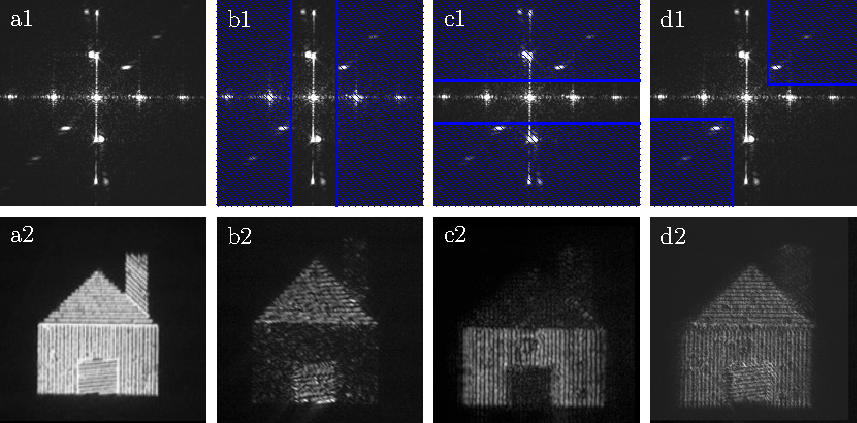
\includegraphics[scale=1]{images/Regina/abb21.pdf}
	
	\caption[Fourierhaus mit verschiedenen Filtern]{
		Durch zwei Schneiden (blau schraffiert) werden verschiedene Teile der Fourierspektren in der Fourierebene herausgefiltert (oben), welches in der Abbildungsebene zum Verschwinden einzelner Teile führt (unten).
	}
	\label{fig:fourierhaus_mit_filtern}
\end{figure}

\subsection{Optische Filterung durch Hochpass-, Tiefpass- und Breitbandfilter}

Als Erstes wird ein Breitbandfilter bei der Zahl vier eingesetzt. Da der Breitbandfilter sowohl kleinere und größere Frequenzen herausfiltert und somit nur eine bestimmtes Frequenzintervall durchlässt, werden die Flächen unterdrückt und Ränder als Doppellinien dargestellt. Beim Breitbandfilter C (Abb %TODO REF!!!
c) konnte dieser Effekt am besten beobachtet werden (Abb.~\ref{fig:vier_mit_breitband}~b). Bei den Breitbandfilter B und A ist die Filterwirkung so stark, dass nur
ein sehr kleiner Frequenzintervall durchgelassen wird und dadurch die Zahl vier kaum noch zu erkennen ist (Abb. \ref{fig:vier_mit_breitband}c, d).

\begin{figure}[h]
	\centering
	%\includegraphicsRS[width=0.4\textwidth]{images/Regina/abb22.jpg}
	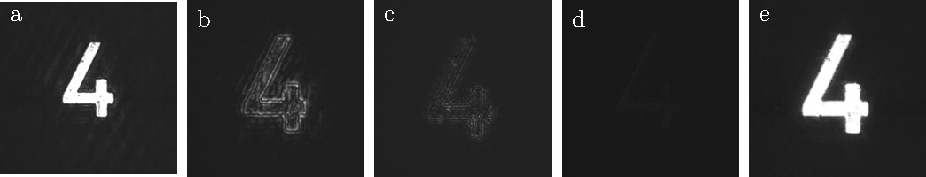
\includegraphics{images/Regina/abb22.pdf}
	\caption[Zahl 4 mit Breitbandfiltern]{
		Die Zahl vier in  der Abbildungsebene ohne Filter (a) und mit dem Breitbandfilter C (b), B (c) und A (d) gefilterte Bilder der Zahl vier.
	}
	\label{fig:vier_mit_breitband}
\end{figure}

Durch die Verwendung eines Tiefpassfilters wurden die niedrigen Frequenzen durchgelassen und somit die hohen Frequenzen herausgefiltert. Diese bewirken eine niedrigere Auflösung des
Bildes, da die Flächen unterdrückt werden, welches in der Abbildung~\ref{fig:vier_mit_breitband}~b dargestellt ist bei der Zahl 4 und dem Buchstaben D dargestellt ist. Da diese beiden Objekte keine innere Flächenstrukturen wie Gitter aufweisen, ist dieser Effekt nicht zu erkennen.
Im Gegenteil dazu wurden bei einem Fingerabdruck ein Hochpassfilter eingesetzt, der die niedrigen Frequenzen herausgefiltert, welches zu einer Heraushebung der Kanten führte (Abb.~\ref{fig:vier_mit_tiefpass}~b). In der Bildverarbeitung werden die Filter eingesetzt und tragen deshalb dort folgende Bezeichnungen: Tiefpass = Weichzeichner und Hochpassfilter = Kantenerkennung.

\begin{figure}[h]
	\centering
	%\includegraphicsRS[width=0.4\textwidth]{images/Regina/abb23.jpg}
	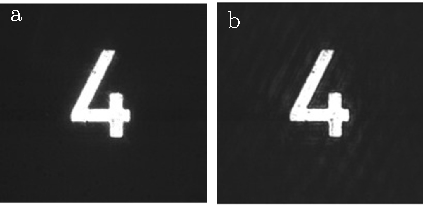
\includegraphics{images/Regina/abb23.pdf}
	\caption[Zahl 4 mit Tiefpassfilter]{
		Die Zahl vier in der Abbildungsebene (a) und mit dem Tiefpassfilter (b) gefilterte Abbildung der Zahl vier.
	}
	\label{fig:vier_mit_tiefpass}
\end{figure}

\begin{figure}[h]
	\centering
	\includegraphicsRS[width=0.4\textwidth]{images/Regina/abb24.jpg}
	\caption[Abbildung Fingerabdruck mit Tiefpassfilter]{Fingerabdruck ohne (a) und mit einem Tiefpassfilter (b)}
	\label{fig:fingerabdruck_mit_filtern}
\end{figure}

\subsection{Schlierenverfahren durch Verwendung eines Halbebenenfilters}

Mit Hilfe eines Halbebenenfilters (Schneide) wurden die durch   eine brennende Kerze erzeugten Schlieren dargestellt (Abb.~\ref{fig:luftstroemungen}). Als Schlieren werden Bereiche bezeichnet, die sich von ihrer Umgebung  in  der  Dichte  bzw.  im  Brechungsindex  unterscheiden,  welche  in  unseren Versuch die durch  die  Kerze erzeugten Luftströmungen darstellten. Bei diesem Versuchsaufbau  wurde  das  Prinzip  genutzt,  dass  parallele  Strahlenbündel  beim  Durchgang durch   ein   inhomogenes Dichtefeld   unterschiedlich   stark   abgelenkt   werden.   Durch   die eingesetzte  Schneide,  wurden  die  Anteile  des  gebrochenen  Lichts  ausgeblendet,  so  dass richtungsabhängige  Brechzahl-  bzw.  Dichtegradienten auf  dem  Projektionsschirm  sichtbar wurden. Dabei ist die Intensitätsverteilung im   Bild   proportional   zum   Quadrat   der Phasenverschiebung   durch   das   Objekt.   Somit   ermöglicht es dieses Verfahren, eine Phasenverschiebung sichtbar zu machen. 

\begin{figure}[h]
	\centering
	\includegraphicsRS[width=0.4\textwidth]{images/Regina/abb25.jpg}
	\caption[Durch Schlierenverfahren sichtbar gemachte Luftströmungen]{
		Durch Schlierenverfahren sichtbar gemachte Luftströmungen (durch Pfeile markiert).
	}
	\label{fig:luftstroemungen}
\end{figure}